\documentclass{article}
\usepackage{hyperref}
\usepackage{listings}
\usepackage{color}
\usepackage{geometry}
\usepackage{graphicx}
\usepackage{amsmath}
\usepackage{caption}
\usepackage{subcaption}
\geometry{margin=1in}
\pdfminorversion=6

\newcommand\TODO[1]{\textcolor{red}{TODO: #1}}

\newcommand\header[2]{
    \begin{center}
        {\large
        UCSD CSE 272 Assignment #1: \\
        \vspace{0.3cm}
        \Large
        #2}
    \end{center}
}

\definecolor{dkgreen}{rgb}{0,0.6,0}
\definecolor{gray}{rgb}{0.5,0.5,0.5}
\definecolor{mauve}{rgb}{0.58,0,0.82}
\lstset{frame=tb,
        aboveskip=3mm,
        belowskip=3mm,
        showstringspaces=false,
        columns=flexible,
        basicstyle={\small\ttfamily},
        numbers=none,
        numberstyle=\tiny\color{gray},
        keywordstyle=\color{blue},
        commentstyle=\color{dkgreen},
        stringstyle=\color{mauve},
        breaklines=true,
        breakatwhitespace=true,
        tabsize=2
}


\begin{document}

\header{2}{Volumetric Path Tracing}

\begin{figure}[h]
    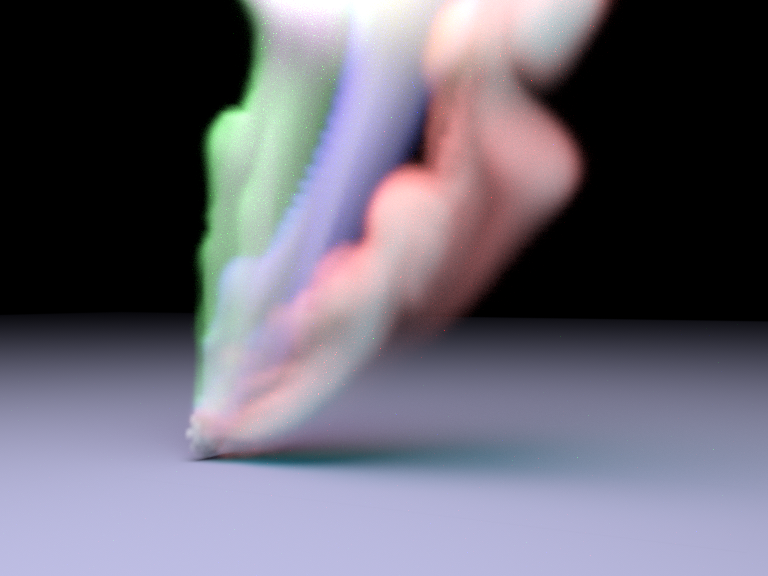
\includegraphics[width=\linewidth]{imgs/colored_smoke.png}
    \caption{The figure shows a heterogeneous volume with a spectrally varying density over space, rendered with multiple-scattering. Smoke data are generated using Wenzel Jakob's \href{http://www.mitsuba-renderer.org/misc.html}{fsolver}.}
    \label{fig:gallery}
\end{figure}

In this homework, we will build a volumetric path tracer that can handle scattering and absorption inside participating media inside lajolla. We will split the development into 6 steps and build 6 volumetric path tracers. Each has more features than the previous ones.\footnote{This approach is inspired by Steve Marschner's \href{https://www.cs.cornell.edu/courses/cs6630/2015fa/notes/10volpath.pdf}{course note} on volumetric path tracing.} Your $n$-th volumetric path tracer should be able to render all scenes the $(n-1)$-th one can handle. If you want, you can only submit the final volumetric path tracer and let all the rest call the final code. This process is for helping you to slowly and steadily build up your rendering algorithm. You will notice that the scores sum up to more than $100\%$. This is because the last volumetric path tracer is a bit more mathematically involved (the implementation is not too bad though), so if you only did the first fifth, you still get $90\%$ of the scores. If you do all of them, you get $110\%$.

\href{https://cs.dartmouth.edu/~wjarosz/publications/novak18monte-sig.html}{This SIGGRAPH course note} is a good reference if you fail to understand the handout. Steve Marschner's course note in the footnote is also very useful. Most of the math in the last part is from Miller et al.~\cite{Miller:2019:NPI} and Georgiev et al.~\cite{Georgiev:2019:IFV}'s articles.

\paragraph{Submission and grading.} Please upload a zip file to Canvas including your code, and a text file (readme.txt) answering the questions below. For the questions, as long as you say something plausible, you will get full scores. As usual, think hard about the questions. We want you to get the high-level concepts correct, rather than trying to match every single detail.

Participating media are volumes with many infinitesimal particles absorbing and scattering lights. Given a ray inside the volume parametrized by distance $\mathbf{p}(t)$, the radiance along the ray is modeled by the \emph{radiative transfer equation}:
\begin{equation}
\frac{\mathrm{d}}{\mathrm{d}t} L(\mathbf{p}(t), \omega) = -(\sigma_a(\mathbf{p}(t)) + \sigma_s(\mathbf{p}(t))) L(\mathbf{p}(t), \omega) + L_e(\mathbf{p}(t), \omega) + \sigma_s(\mathbf{p}(t)) \int_{S^2} \rho(\mathbf{p}(t), \omega, \omega') L(\mathbf{p}(t), \omega') \mathrm{d}\omega',
\label{eq:rte}
\end{equation}
where $L$ is the radiance, $\sigma_a$ is the \emph{absorption coefficient}, $\sigma_s$ is the \emph{scattering coefficient}, $L_e$ is the (volumetric) emission, $\rho$ is the \emph{phase function} that is akin to BSDFs in surface rendering, and $S^2$ is the spherical domain.

This looks a bit scary, so let's break it down. For now, we'll drop the arguments for $\sigma_a$ and $\sigma_s$, but in general, they can still be spatially varying. The radiative transfer equation is made of four components: \textbf{absorption}, \textbf{emission}, \textbf{in-scattering}, and \textbf{out-scattering}. Absorption and emission handle particles that absorb and emit lights\footnote{Some text will formulate the emission as $\frac{\mathrm{d}}{\mathrm{d}t} L_a(\mathbf{p}(t), \omega) = \sigma_a L_e(\mathbf{p}(t), \omega)$. This is effectively the same with a slight reparameterization $L_e \rightarrow \sigma_a L_e$.}:
\begin{equation}
\frac{\mathrm{d}}{\mathrm{d}t} L_a(\mathbf{p}(t), \omega) = -\sigma_a L_a(\mathbf{p}(t), \omega) + L_e(\mathbf{p}(t), \omega).
\end{equation}
Notice how this is a linear ordinary differential equation $x' = ax + b$, where $\sigma_a$ attenuates lights and $L_e$ is the gain.

The in-scattering accounts for all the lights bounce between the particles along the ray, just like the surface rendering equation:
\begin{equation}
\frac{\mathrm{d}}{\mathrm{d}t} L_{is}(\mathbf{p}(t), \omega) = \sigma_s \int_{S^2} \rho(\mathbf{p}(t), \omega, \omega') L(\mathbf{p}(t), \omega') \mathrm{d}\omega'.
\end{equation}

However, the light does not just bounce \emph{into} the ray, it also bounces \emph{out}. That's what the out-scattering considers:
\begin{equation}
\frac{\mathrm{d}}{\mathrm{d}t} L_{os}(\mathbf{p}(t), \omega) = -\sigma_s L_{os}(\mathbf{p}(t)).
\end{equation}

Combining all these components, we get the full radiative transfer equation (Equation~\ref{eq:rte}). Notice that the full radiative transfer equation is also like a linear ODE: $-(\sigma_a + \sigma_s) L$ attenuates light, and $L_e$ and the spherical integral are the gain that makes things brighter. For this reason, we often let $\sigma_t = \sigma_a + \sigma_s$ and call it the \emph{extinction coefficient}.

We'll start from a simplified version of the radiative transfer equation, then slowly handle more complex situations. To make things simpler, we will throughout assume our medium does not emit light itself: it will receive lighting from other surfaces in the scene.

Before that, let's introduce lajolla's data structures for storing the participating media.

\section{Lajolla's participating media data structures and interfaces}
\begin{figure}
    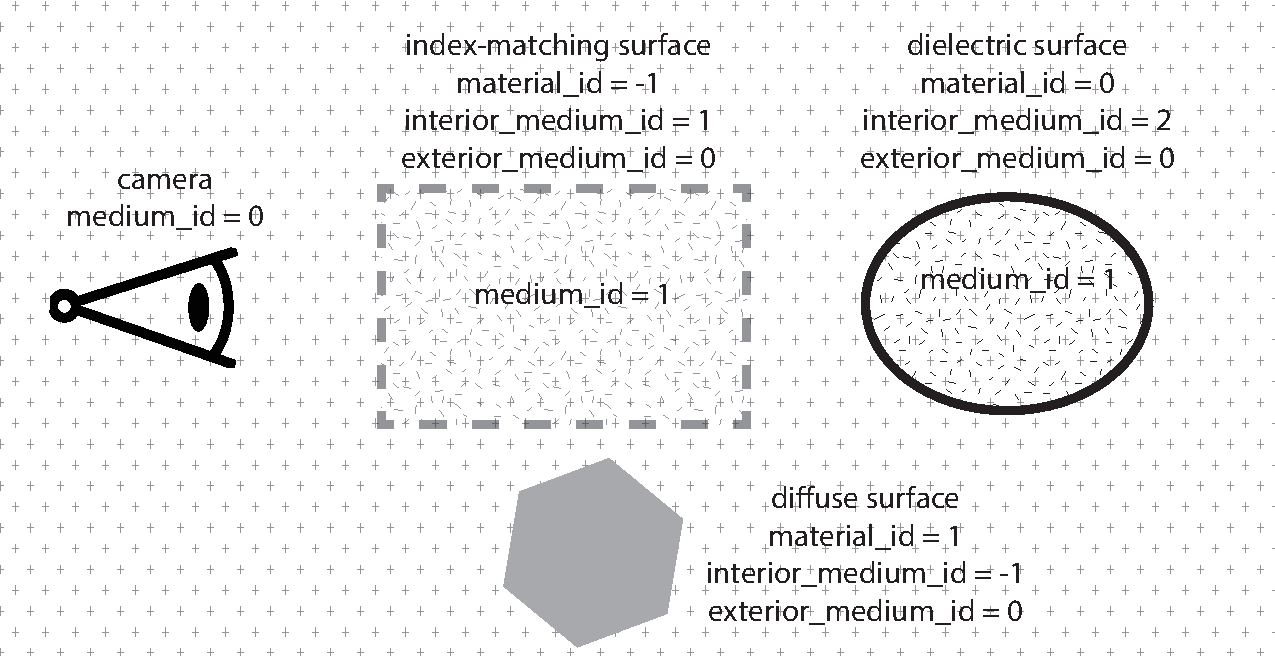
\includegraphics[width=\linewidth]{imgs/media.pdf}
    \caption{Lajolla assumes that media are separated by closed surface boundaries. At the object surface, we store the ID of the interior and exterior media (if both of them are vacuum, set the ID to \lstinline{-1}). The outmost medium is specified at the camera (and can be accessed through \lstinline{camera.medium_id}). A surface can be \emph{index-matching} meaning that light passes through without changing direction or losing energy. In this case, the \lstinline{material_id} of the surface is set to \lstinline{-1}. A surface can also be transmissive. In this case, it is assigned a transmissive material like \lstinline{roughdielectric}.}
    \label{fig:data_structure}
\end{figure}

\paragraph{The Medium struct in lajolla.} Lajolla's medium interface is for querying the media parameters $\sigma_a$, $\sigma_s$, phase function $\rho$, and the \emph{majorant} which is the upper bound of the extinction coefficient $\sigma_t = \sigma_a + \sigma_s$ -- we will need the majorant in our final renderer. 
\begin{lstlisting}[language=c++]
struct MediumBase {
    PhaseFunction phase_function;
};

struct HomogeneousMedium : public MediumBase {
    Spectrum sigma_a, sigma_s;
};

struct HeterogeneousMedium : public MediumBase {
    VolumeSpectrum albedo, density;
};

using Medium = std::variant<HomogeneousMedium, HeterogeneousMedium>;

/// the maximum of sigma_t = sigma_s + sigma_a over the whole space
Spectrum get_majorant(const Medium &medium, const Ray &ray);
Spectrum get_sigma_s(const Medium &medium, const Vector3 &p);
Spectrum get_sigma_a(const Medium &medium, const Vector3 &p);

inline PhaseFunction get_phase_function(const Medium &medium) {
    return std::visit([&](const auto &m) { return m.phase_function; }, medium);
}
\end{lstlisting}
You will need these functions to obtain the necessary quantities in the homework.

A \lstinline{HomogeneousMedium} should be straightforward: it contains constant $\sigma_a$ and $\sigma_s$.
We will talk more about \lstinline{HeterogeneousMedium} and \lstinline{PhaseFunction} later.

Lajolla assumes that the media are separated by surface boundaries (Figure~\ref{fig:data_structure}). It's up to the upstream users to make sure they are consistent with each other, and the surfaces are closed (if they are not, the results are undefined).\footnote{Modern production volume renderers have paid special attention to make sure the renderers can handle all sorts of inputs, including nested volumes. See \href{https://graphics.pixar.com/library/ProductionVolumeRendering/index.html}{here} for more information.}

In the scene file, each objects are marked with corresponding exterior and interior media:
\begin{lstlisting}[language=xml]
    <medium type="homogeneous" id="medium">
        <rgb name="sigmaA" value="0.5 0.5 0.5"/>
        <rgb name="sigmaS" value="0.0 0.0 0.0"/>
        <float name="scale" value="3"/>
    </medium>

    <shape type="sphere">
        <!-- ...  -->
        <ref name="exterior" id="medium"/>
    </shape>

    <sensor type="perspective">
        <!-- ... -->

        <ref id="medium"/>
    </sensor>
\end{lstlisting}
If an object has the same interior and exterior media, then it does not need to specify them. 

The \lstinline{Medium}s are stored in \lstinline{scene.media} which you can access through \lstinline{scene.media[medium_id]}. The \lstinline{intersection} routine in lajolla returns a \lstinline{PathVertex} object which contains relevant information of the intersection:
\begin{lstlisting}[language=c++]
struct PathVertex {
    Vector3 position;
    Vector3 geometry_normal;
    // ...
    int shape_id = -1;
    int primitive_id = -1; // For triangle meshes. This indicates which triangle it hits.
    int material_id = -1;

    // If the path vertex is inside a medium, these two IDs
    // are the same.
    int interior_medium_id = -1;
    int exterior_medium_id = -1;
};
\end{lstlisting}

\section{Single monochromatic absorption-only homogeneous volume}
\begin{figure}
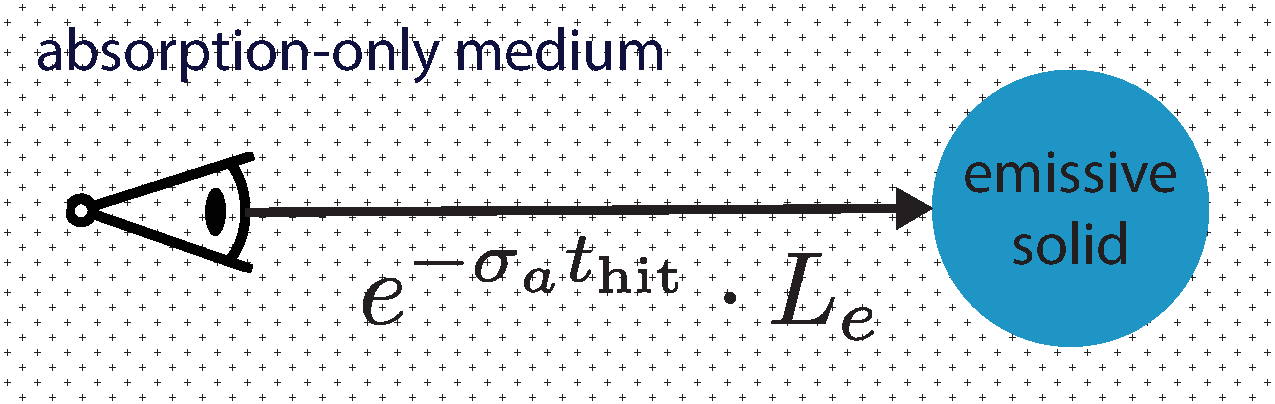
\includegraphics[width=\linewidth]{imgs/absorption_medium.pdf}
\caption{The setup of our first volumetric renderer.}
\label{fig:volpath1_illustration}
\end{figure}

Our first volume renderer will make four assumptions.
\begin{itemize}
    \item There is only a single, homogeneous ($\sigma_a$ and $\sigma_s$ are constants over space) volume.
    \item The volume does not scatter light: $\sigma_s = 0$.
    \item The surfaces in the scene only emit lights (with intensity $L_e$) and do not reflect/transmit lights.
    \item The volume is monochromatic: the three color channels of $\sigma_s$ and $\sigma_a$ have the same values.
\end{itemize}

Under these assumptions, the radiative transfer equation becomes
\begin{equation}
\frac{\mathrm{d}}{\mathrm{d}t} L_1(\mathbf{p}(t), \omega) = -\sigma_a L_1(\mathbf{p}(t), \omega),
\end{equation}
and we know $L_1(\mathbf{p}(t_{\text{hit}}), \omega) = L_e(\mathbf{p}(t_{\text{hit}}))$ where $t_{\text{hit}}$ is the distance between the origin of the ray and the emissive surface.

This ordinary differential equation has a simple closed-form:
\begin{equation}
L_1(\mathbf{p}(0), \omega) = \exp\left(-\sigma_a t_{\text{hit}} \right) L_e(\mathbf{p}(t_{\text{hit}})).
\end{equation}
Figure~\ref{fig:volpath1_illustration} illustrates the setup. In volume rendering the exponential term
$\exp\left(-\sigma_a t_{\text{hit}} \right)$ is often called the ``transmittance''.

Our rendering algorithm (that generates a sample for a pixel) is as follows (in Python-style pseudo-code).
\begin{lstlisting}[language=python]
def L(screen_pos, rng):
  camera_ray = sample_primary(camera, screen_pos, rng)
  isect = intersect(scene, camera_ray)
  if isect:
    transmittance = exp(-sigma_a * t)
    Le = 0
    if is_light(isect):
      Le = isect.Le
    return transmittance * Le
  return 0
\end{lstlisting}

While our volumes are monochromatic, the light can be colored, so the final results can still have color.

\begin{figure}
\centering
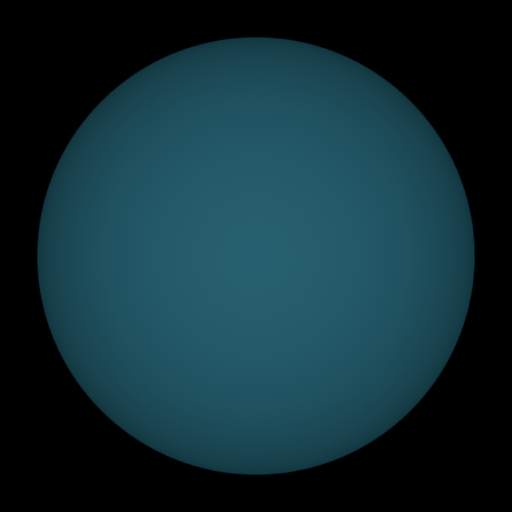
\includegraphics[width=0.5\linewidth]{imgs/volpath_1.png}
\caption{How Figure~\ref{fig:volpath1_illustration} would be rendered like.}
\label{fig:volpath1}
\end{figure}

\paragraph{Question(s) (8\%).} 
Answer these questions in a text file:
\begin{enumerate}
    \item Change the absorption parameters to zero in \lstinline{scenes/volpath_test/volpath_test1.xml}. What do you see? Why?
    \item In the homework, we assume the volume being not emissive. If you were tasked to modify the pseudo code above to add volume emission, how would you do it? Briefly describe your approach.
\end{enumerate}
Think about these questions as you write the code.

\paragraph{Task (10\%).} You will implement the algorithm above in the \lstinline{vol_path_tracing_1} function in \lstinline{vol_path_tracing.h}. You might want to first look at the surface path tracing code in \lstinline{path_tracing.h} to understand lajolla's API better. Test your rendering using the scene \lstinline{scenes/volpath_test/volpath_test1.xml}. You should get an image that looks like Figure~\ref{fig:volpath1}.

\paragraph{Ray differentials.} In the surface path tracer, lajolla uses ray differential for texture lookup. Determining ray differentials for volumetric scattering is an unsolved problem. For this homework, we will disable ray differentials by setting it to 0 and do not change it:
\begin{lstlisting}[language=c++]
RayDifferential ray_diff = RayDifferential{Real(0), Real(0)};
\end{lstlisting}

\paragraph{Environment maps.} Throughout the homework, we assume there is no environment map in the scene. 

\section{Single monochromatic homogeneous volume with absorption and single-scattering, no surface lighting}
\begin{figure}
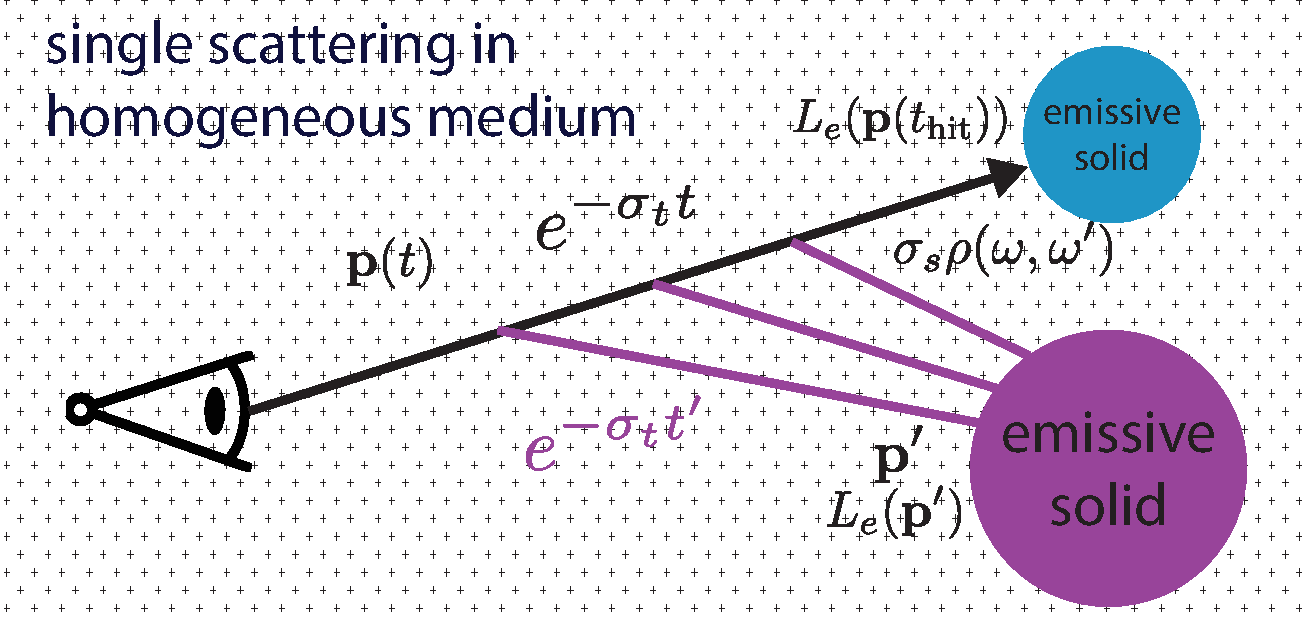
\includegraphics[width=\linewidth]{imgs/single_scattering.pdf}
\caption{The figure shows the setup of our second volumetric renderer. Light can now scatter inside the medium once, and we need to account for the phase function $\rho$ and the extra transmittance $\exp{-\sigma_t t'}$ We need to integrate over the camera ray to account for all scattering.}
\label{fig:volpath2_illustration}
\end{figure}

Our next renderer adds single scattering to the volume (Figure~\ref{fig:volpath2_illustration}). We still assume:
\begin{itemize}
    \item There is only a single, homogeneous ($\sigma_a$ and $\sigma_s$ are constants over space) volume.
    \item The surfaces in the scene only emit lights (with intensity $L_e$) and do not reflect/transmit lights.
    \item The volume is monochromatic: the three color channels of $\sigma_s$ and $\sigma_a$ have the same values.
    \item Light only scatters (changes direction) once in the volume.
\end{itemize}

Now we need to solve the radiative transfer equation (Equation~\ref{eq:rte}), except the spherical integral only recurse once:
\begin{equation}
L_{\text{scatter}1}(\mathbf{p}, \omega) = \int_{\mathcal{M}} \rho(\mathbf{p}(t), \omega, \omega') L_e(\mathbf{p}', \omega') \exp\left(-\sigma_t \left\| \mathbf{p}(t) - \mathbf{p}' \right\|\right) \frac{\left| \omega' \cdot \mathbf{n}_{\mathbf{p}'} \right|}{{\left\| \mathbf{p}(t) - \mathbf{p}' \right\|}^2} \text{visible}(\mathbf{p}(t), \mathbf{p}') \mathrm{d}\mathbf{p}',
\end{equation}
instead of integrating over the sphere $S^2$, we apply a change of variable to integrate over the scene manifold $\mathcal{M}$ for all points on surfaces $\mathbf{p}'$. $\frac{\left| \omega' \cdot \mathbf{n}_{\mathbf{p}'} \right|}{{\left\| \mathbf{p}(t) - \mathbf{p}' \right\|}^2} \text{visible}(\mathbf{p}(t), \mathbf{p}')$ is the Jacobian of the transformation and $\omega' = \frac{\mathbf{p}' - \mathbf{p}(t)}{\left\| \mathbf{p}' - \mathbf{p}(t) \right\|}$. $\exp\left(-\sigma_t \left\| \mathbf{p}(t) - \mathbf{p}' \right\|\right)$ is the transmittance between $\mathbf{p}(t)$ and $\mathbf{p}'(t)$ that represents energy loss due to absorption and out-scattering (hence it uses the extinction coefficient $\sigma_t = \sigma_a + \sigma_s$ instead of $\sigma_a$ or $\sigma_s$). $s1$ stands for ``scattering once''.

The radiative transfer equation is then
\begin{equation}
\frac{\mathrm{d}}{\mathrm{d}t} L_2(\mathbf{p}(t), \omega) = -\sigma_t L_2(\mathbf{p}(t), \omega) + \sigma_s L_{\text{scatter}1}(\mathbf{p}, \omega).
\label{eq:rte_single_scattering}
\end{equation}

We no longer have a simple closed-form solution and resort to Monte Carlo sampling. To make the differential equation more familiar to us who are more used to Monte Carlo rendering, let's convert the equation above into an integral:
\begin{equation}
L_2(\mathbf{p}(0), \omega) = \int_{0}^{t_{\text{hit}}} \exp\left(-\sigma_t t \right) \sigma_s L_{\text{scatter}1}(\mathbf{p}, \omega) \mathrm{d}t + \exp\left(-\sigma_t t_{\text{hit}} \right) L_e(\mathbf{p}(t_{\text{hit}}))
\label{eq:rte_single_scattering_integral_form}
\end{equation}

To sample this integral, we importance sample the transmittance $\exp\left(-\sigma_t t\right)$. To do this we need to sample a distance $t$ such that $p(t) \propto \exp\left(-\sigma_t t\right)$. This can be done by the standard inverse tranform sampling. We first integrate $\exp\left(-\sigma_t t \right)$:
\begin{equation}
\int_{0}^{t} \exp\left(-\sigma_t s\right) \mathrm{d}s = -\frac{exp(-\sigma_t * t)}{\sigma_t} + \frac{1}{\sigma_t}.
\end{equation}
We thus know that $p(t) = \sigma_t\exp\left(-\sigma_t t\right)$ (why?). 
Integrating $p(t)$ to get the CDF we get
\begin{equation}
T_{\text{exp}}^{-1}(t) = -\exp\left(-\sigma_t * t\right) + 1 = u.
\end{equation}
Inverting $T_{\text{exp}}^{-1}$ we get
\begin{equation}
t = \frac{\log\left(1 - u\right)}{-\sigma_t}.
\end{equation}

Now, note that our integral is only in $[0, t_{\text{hit}}]$. Our sampling above can generate $t > t_{\text{hit}}$. In this case, we hit a surface and account for the surface emission $L_e(\mathbf{p}(t_{\text{hit}}))$ in Equation~\ref{eq:rte_single_scattering_integral_form}. We need to account for the probability of that:
\begin{equation}
P(t \geq t_{\text{hit}}) = \int_{t_{\text{hit}}}^{\infty} \sigma_t\exp\left(-\sigma_t t\right) = \exp\left(-\sigma_t * t_{\text{hit}}\right)
\label{eq:hit_surface_prob}
\end{equation}

Thus our rendering algorithm (that generates a sample for a pixel) looks like this:
\begin{lstlisting}[language=python]
def L(screen_pos, rng):
  camera_ray = sample_primary(camera, screen_pos, rng)
  isect = intersect(scene, camera_ray)

  u = next(rng) # u \in [0, 1]
  t = -log(1 - u) / sigma_t
  if t < isect.t_hit:
    trans_pdf = exp(-sigma_t * t) * sigma_t
    transmittance = exp(-sigma_t * t)
    # compute L_s1 using Monte Carlo sampling
    p = camera_ray.org + t * camera_ray.dir
    # Equation 7
    L_s1_estimate, L_s1_pdf = L_s1(p, sample_point_on_light(rng))
    return (transmittance / trans_pdf) * sigma_s * (L_s1_estimate / L_s1_pdf)
  else:
    # hit a surface, account for surface emission
    trans_pdf = exp(-sigma_t * isect.t_hit)
    transmittance = exp(-sigma_t * isect.t_hit)
    Le = 0
    if is_light(isect):
      Le = isect.Le
    return (transmittance / trans_pdf) * Le
\end{lstlisting}

\begin{figure}
\centering
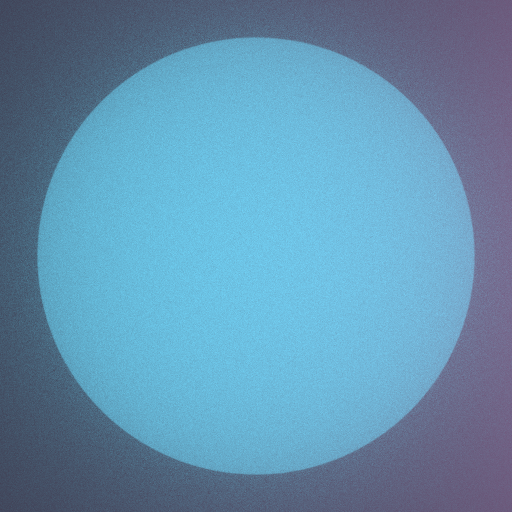
\includegraphics[width=0.5\linewidth]{imgs/volpath_2.png}
\caption{How a scene like the setup in Figure~\ref{fig:volpath2_illustration} would be rendered like. Now there is scattering, the area surrounding the solid sphere can have non-zero radiance.}
\label{fig:volpath2}
\end{figure}

\paragraph{Question(s) (8\%).} 
Answer these questions in a text file:
\begin{enumerate}
    \item In the derivation above, how did we get from $p(t) \propto \exp(-\sigma_t t)$ to $p(t) = \sigma_t \exp(\sigma_t t)$? 
    \item How was Equation~\eqref{eq:hit_surface_prob} incorporated into the pseudo code above? Why is it done this way?
    \item Play with the parameters $\sigma_s$ and $\sigma_a$, how do they affect the final image? Why? (we assume monochromatic volumes, so don't set the parameters to be different for each channel.)
    \item Change the phase function from isotropic (the default one) to Henyey-Greenstein by uncommenting the phase function specification in the scene \lstinline{scenes/volpath_test/volpath_test2.xml}. Play with the parameter $g$ (the valid range is $(-1, 1)$). What does $g$ mean? How does the $g$ parameter change the appearance? Why?
\end{enumerate}

\paragraph{Task (10\%).} You will implement the algorithm above in the \lstinline{vol_path_tracing_2} function in \lstinline{vol_path_tracing.h}. For evaluating the phase function $\rho$, use the \lstinline{eval} function in \lstinline{phase_function.h}.
Test your rendering using the scene \lstinline{scenes/volpath_test/volpath_test2.xml}. You should get an image that looks like Figure~\ref{fig:volpath2}. Note that the rendered image will be a bit noisy even a high sampling count. This is expected, since we are not importance sampling the geometry term $\frac{\left| \omega' \cdot \mathbf{n}_{\mathbf{p}'} \right|}{{\left\| \mathbf{p}(t) - \mathbf{p}' \right\|}^2} \text{visible}(\mathbf{p}(t), \mathbf{p}')$ along $t$. Such importance sampling scheme is called the \emph{equiangular sampling}~\cite{Rief:1984:TLE,Kulla:2012:IST}. Equiangular sampling is out of the scope for this homework, but you're free to implement it!

\paragraph{Bonus (25\%).} Implement the \emph{equiangular sampling}~\cite{Kulla:2012:IST} sampling strategy. Potentially combine it with the transmittance sampling using multiple importance sampling. (I do not recommend you implement this until you've finished the whole homework.) If you implement this bonus, please mention it in the README file, and provide rendering comparisons.

\section{Multiple monochromatic homogeneous volumes with absorption and multiple-scattering using only phase function sampling, no surface lighting}
\begin{figure}
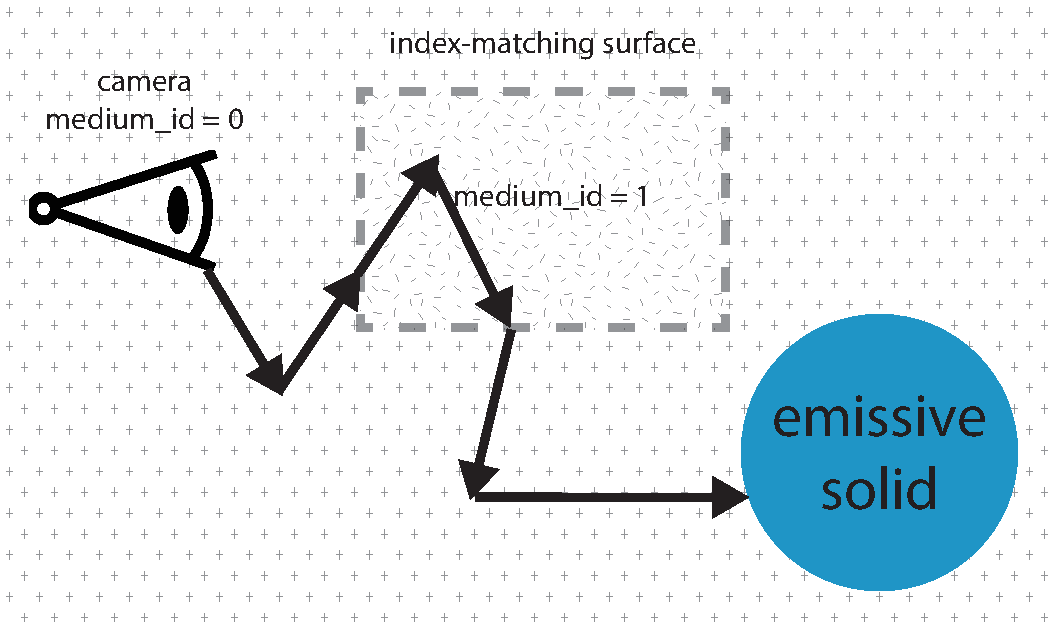
\includegraphics[width=\linewidth]{imgs/multiple_scattering.pdf}
\caption{Setup of our third volumetric renderer.}
\label{fig:volpath3_illustration}
\end{figure}
Our next volumetric path tracer would start to be a bit complicated. This time we will consider multiple scattering between multiple volumes (Figure~\ref{fig:volpath3_illustration}). We make the following assumptions:
\begin{itemize}
    \item There are multiple homogeneous ($\sigma_a$ and $\sigma_s$ are constants over space) volumes.
    \item The surfaces in the scene only emit lights (with intensity $L_e$) and do not reflect/transmit lights.
    \item The volume is monochromatic: the three color channels of $\sigma_s$ and $\sigma_a$ have the same values.
    \item Light can scatter (changes direction) multiple times in the volume, but we only sample the scattering by sampling the phase function $\rho$.
\end{itemize}

Under this assumption, our volumetric integral becomes:
\begin{equation}
L_3(\mathbf{p}(0), \omega) = \int_{0}^{t_{\text{hit}}} \exp\left(-\sigma_t t \right) \sigma_s L_{\text{scatter}}(\mathbf{p}, \omega) \mathrm{d}t + \exp\left(-\sigma_t t_{\text{hit}} \right) L_e(\mathbf{p}(t_{\text{hit}})),
\label{eq:rte_multiple_scattering_integral_form}
\end{equation}
where $L_{\text{scatter}}$ is recursive:
\begin{equation}
L_{\text{scatter}}(\mathbf{p}, \omega) = \int_{S^2} \rho(\mathbf{p}(t), \omega, \omega') L_3(\mathbf{p}(t), \omega') \mathrm{d}\omega'.
\end{equation}

Our strategy of sampling the integral $L_3$ is as follows: we first generate a distance $t$ by sampling the transmittance as previous. If $t < t_{\text{hit}}$, we need to evaluate $L_{\text{scatter}}$. We do so by sampling the phase function $\rho$ for a direction $\omega'$. We then sample the next distance for evaluating the $L_3$ inside the $S^2$ integral. If we hit a surface ($t' \geq t'_{\text{hit}}$ for some distance $t'$ along our sampling), we include the emission $L_e$ and terminate.

\paragraph{Number of bounces.} We use the \lstinline{scene.options.max_depth} parameter to control the number of bounces. If \lstinline{max_depth = -1}, then we can bounce infinite amount of time. Otherwise, a light path can have at most \lstinline{max_depth + 1} vertices, including the camera vertex and the light vertex. \lstinline{max_depth = 2} corresponds to the single scattering case in the previous section.

\paragraph{Index-matched surfaces.} Sometimes we will hit surfaces that have no materials assigned (\lstinline{material_id = -1}). For these surfaces, we need to pass through them. Passing through an index-matched surface counts as one bounce.

\paragraph{Russian roulette.} We use the \lstinline{scene.options.rr_depth} to control the Russian roulette behavior. We initialize Russian roulette when a light path has \lstinline{rr_depth + 1} vertices. We set the probability for termination to
\begin{equation}
P_{rr} = \min\left(\frac{\text{contrib}(\text{path})}{p(\text{path})}, 0.95\right),
\end{equation}
where $\text{contrib}(path)$ is the evaluation of the integrand of the path in the volumetric integral, and $p(\text{path})$ is the probability density of generating such path.

The pseudo code looks like this:
\begin{lstlisting}[language=python]
def L(screen_pos, rng):
  ray = sample_primary(camera, screen_pos, rng)
  current_medium = camera.medium

  current_path_throughput = 1
  radiance = 0
  bounces = 0
  while True
    scatter = False
    isect = intersect(scene, ray)
    # isect might not intersect a surface, but we might be in a volume
    transmittance = 1
    trans_pdf = 1
    if current_medium:
      # sample t s.t. p(t) ~ exp(-sigma_t * t)
      # compute transmittance and trans_pdf
      # if t < t_hit, set scatter = True
      # ...
      ray.org = ray.org + t * ray.dir
    
    current_path_throughput *= (transmittance / trans_pdf)
    if not scatter:
      # reach a surface, include emission
      radiance += current_path_throughput * Le(isect)

    if bounces == max_depth - 1 and max_depth != -1:
      # reach maximum bounces
      break

    if not scatter and isect:
      if isect.material_id == -1:
        # index-matching interface, skip through it
        current_medium = update_medium(ray, isect, medium)
        bounces += 1
        continue

    # sample next direct & update path throughput
    if scatter:
      next_dir = sample_phase_function(-ray.dir, rng)
      current_path_throughput *=
        (phase_function(-ray.dir, next_dir) / sample_phase_pdf(-ray.dir, next_dir)) * sigma_s
      # update ray.dir
      # ...
    else:
      # Hit a surface -- don't need to deal with this yet
      break
    
    # Russian roulette
    rr_prob = 1
    if (bounces >= rr_depth):
      rr_prob = min(current_path_throughput, 0.95)
      if next(rng) > rr_prob:
        break
      else:
        current_path_throughput /= rr_prob
    bounces += 1
  return radiance
\end{lstlisting}

The pseudocode relies on the \lstinline{update_medium} routine, which updates the current medium the ray lies in:
\begin{lstlisting}[language=python]
def update_medium(isect, ray, medium):
    if (isect.interior_medium != isect.exterior_medium):
        # At medium transition. Update medium.
        if dot(ray.dir, isect.geometry_normal) > 0:
            medium = isect.exterior_medium_id
        else:
            medium = isect.interior_medium_id
    return medium
\end{lstlisting}
We only update the medium if the intersection specifies a ``medium transition'', where the interior medium
is different from the exterior medium.

\begin{figure}
\centering
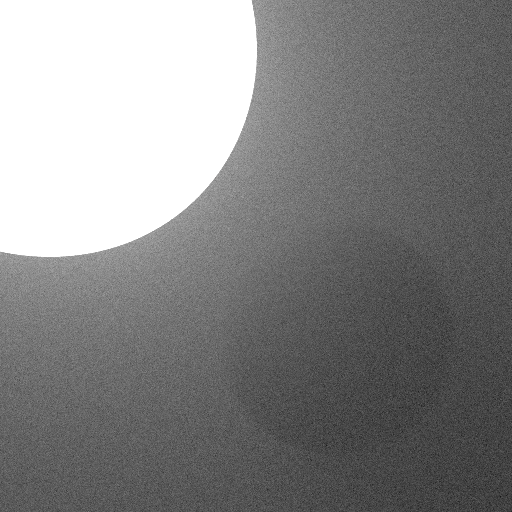
\includegraphics[width=0.5\linewidth]{imgs/volpath_3.png}
\caption{How Figure~\ref{fig:volpath3_illustration} would be rendered like. Left top is a light source, and bottom right is a volume with index-matched interface.}
\label{fig:volpath3}
\end{figure}

\paragraph{Question(s) (8\%).}
Answer these questions in a text file:
\begin{enumerate}
    \item Play with the parameters $\sigma_s$, $\sigma_a$ of different volumes, and change \lstinline{max_depth}, how do they affect the final image?
    How does increasing/decreasing $\sigma_s$ and $\sigma_a$ of \lstinline{medium1} and \lstinline{medium2} affect the appearance, respectively?
    Why?
    Do different $\sigma_s$ and $\sigma_a$ values affect how high you should set \lstinline{max_depth}?
    \item Switch to the Henyey-Greenstein phase function again. How does changing the $g$ parameter affect the appearance? Why?
    \item Propose a phase function yourself (don't have to describe the exact mathematical form). How would you design the shape of the phase function? What parameter would you set to control it?
\end{enumerate}
Think about these questions as you write the code.

\paragraph{Task (10\%).} You will implement the algorithm above in the \lstinline{vol_path_tracing_3} function in \lstinline{vol_path_tracing.h}. For sampling the phase function $\rho$, use the \lstinline{sample_phase_function} and \lstinline{pdf_sample_phase} functions in \lstinline{phase_function.h}.
Test your rendering using the scene \lstinline{scenes/volpath_test/volpath_test3.xml}. You should get an image that looks like Figure~\ref{fig:volpath3}. Again, the image can be a bit noisy since we have not implemented next event estimation.

\section{Multiple monochromatic homogeneous volumes with absorption and multiple-scattering with both phase function sampling and next event estimation, no surface lighting}

\begin{figure}
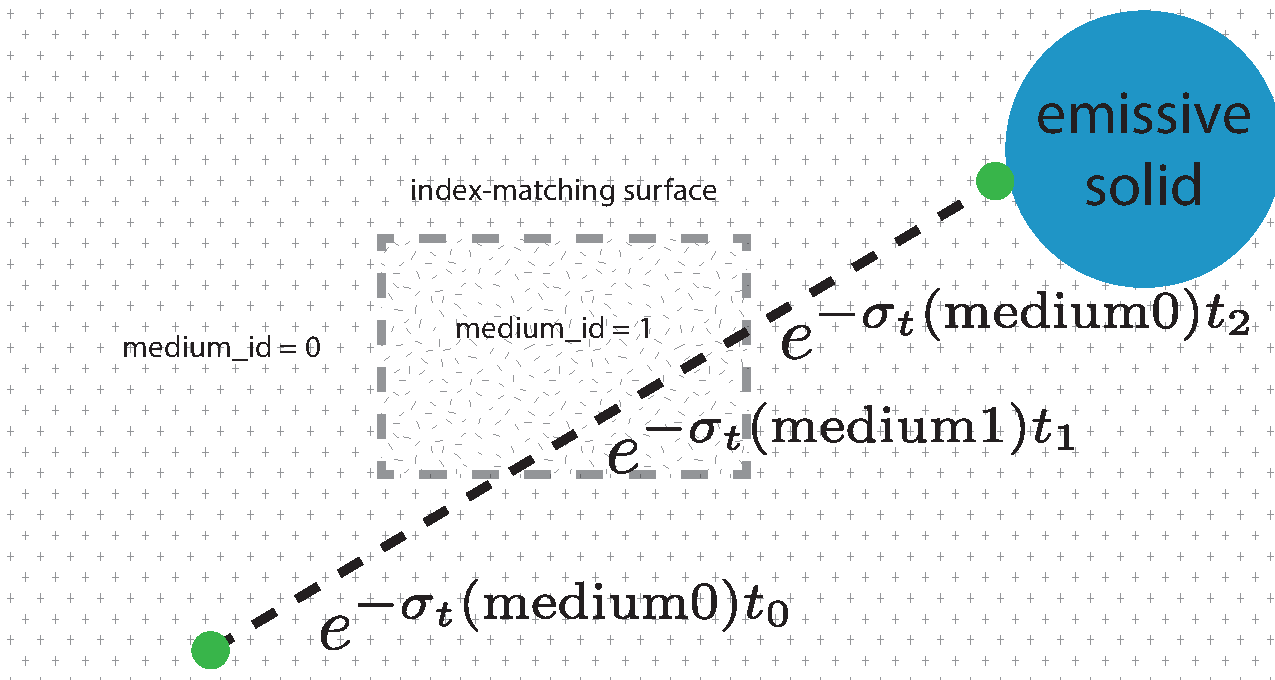
\includegraphics[width=\linewidth]{imgs/volume_next_event_estimation.pdf}
\caption{Our 4th volumetric path tracer adds next event estimation to the previous one. Given a point in the volume, we first select a point on the light, then we trace a shadow ray towards the light. Unlike normal next event estimation, where the visibility is a binary function, here the visibility is determined by the transmittance between the volume point and the light source. Our shadow ray needs to trace through index-matching surfaces and skip through them, accounting for the transmittance of all the media in between.}
\label{fig:volpath4_illustration}
\end{figure}

Sampling only using the phase function is inefficient, especially when the light source is relatively small. Our fourth volumetric path tracer adds the next event estimation to the sampling (Figure~\ref{fig:volpath4_illustration}) as our section title grows out of control. Instead of sampling from the phase function, we pick a point on the light source, and trace a shadow ray towards the light to account for the transmittance in between. We also need to account for \emph{index-matching surfaces} -- surfaces that don't have a material assigned to them (so the index of refraction is the same inside and outside). Our shadow ray will pass through all index-matching surfaces and account for all the transmittance in between.

Mathematically, the next event estimation is a change of variable of the spherical single scattering integral:
\begin{equation}
\int_{S^2} \rho(\mathbf{p}, \omega, \omega') T(\mathbf{p}, \mathbf{p}') L_e(\mathbf{p}') \mathrm{d} \omega' =
\int_{E} \rho(\mathbf{p}, \omega, \omega') T(\mathbf{p}, \mathbf{p}') L_e(\mathbf{p}') \frac{\left|\omega' \cdot \mathbf{n}_{\mathbf{p}'}\right|}{\left|\mathbf{p} - \mathbf{p}'\right|^2} \mathrm{d} \mathbf{p}',
\end{equation}
where $\mathbf{p}'$ are points on the light sources, $T(\mathbf{p}, \mathbf{p}')$ is the transmittance between point $\mathbf{p}$ and $\mathbf{p}'$. We also need to include the geometry term $\frac{\left|\omega' \cdot \mathbf{n}_{\mathbf{p}'}\right|}{\left|\mathbf{p} - \mathbf{p}'\right|^2}$ as the Jacobian of the change of variable.

The pseudo-code for the volumetric next event estimation looks like this:
\begin{lstlisting}[language=python]
def next_event_estimation(p, current_medium):
    p_prime = sample_point_on_light(p)
    # Compute transmittance to light. Skip through index-matching shapes.
    T_light = 1
    shadow_medium = current_medium
    shadow_bounces = 0
    p_trans_dir = 1 # for multiple importance sampling
    while True:
      shadow_ray = Ray(p, p_prime - p)
      isect = intersect(scene, shadow_ray)
      next_t = distance(p, p_prime)
      if isect:
        next_t = distance(p, isect.position)
      # Account for the transmittance to next_t
      if shadow_medium:
        T_light *= exp(-sigma_t * next_t)
        p_trans_dir *= exp(-sigma_t * next_t)

      if not isect:
        # Nothing is blocking, we're done
        break
      else:
        # Something is blocking: is it an opaque surface?
        if isect.material_id >= 0:
          # we're blocked
          return 0
        # otherwise, it's an index-matching surface and
        # we want to pass through -- this introduces
        # one extra connection vertex
        shadow_bounces += 1
        if max_depth != -1 and bounces + shadow_bounces + 1 >= max_depth:
          # Reach the max no. of vertices
          return 0

        shadow_medium = update_medium(isect, ray, shadow_medium)
        p = p + next_t * dir_light

    if T_light > 0:
      # Compute T_light * G * rho * L & pdf_nee
      # ...
      contrib = T_light * G * rho * L / pdf_nee
      # Multiple importance sampling: it's also possible
      # that a phase function sampling + multiple exponential sampling
      # will reach the light source.
      # We also need to multiply with G to convert phase function PDF to area measure.
      pdf_phase = pdf_sample_phase(phase_function, dir_view, dir_light) * G * p_trans_dir
      # power heuristics
      w = (pdf_nee * pdf_nee) / (pdf_nee * pdf_nee + pdf_phase * pdf_phase)
      return w * contrib
    return 0
\end{lstlisting}

Then we can put \lstinline{next_event_estimation()} in our previous code and include its contribution. Remember to multiply the result of next event estimation with the transmittance from the previous path vertex to $p$ and $\sigma_s(\mathbf{p})$.

Next, we need to include the multiple importance sampling weight for phase function sampling as well. Previously we included those contribution whenever our path hits a light source:
\begin{lstlisting}[language=python]
    if not scatter:
      # reach a surface, include emission
      radiance += current_path_throughput * Le(isect)
\end{lstlisting}

This time, we need to multiply the contribution with the multiple importance sampling weight $\frac{p_{\text{phase}}^2}{p_{\text{phase}}^2 + p_{\text{nee}}^2}$ -- how do we get those values? The problem is that the quantities that are required for computing these two PDFs might exist several bounces ago, since in our main loop in \lstinline{L} we skip through index-matching surfaces. My strategy for resolving this is to cache the necessary quantities during the main loop. We introduce the quantities \lstinline{dir_pdf} (the pdf of the latest phase function sampling), \lstinline{nee_p_cache} (the last position p that can issue a next event estimation -- if it's on an index-matching surface, it can't issue next event estimation). \lstinline{multi_trans_pdf} (the product PDF of transmittance sampling going through several index-matching surfaces from the last phase function sampling):
\begin{lstlisting}[language=python]
def L(screen_pos, rng):
  # ...
  current_path_throughput = 1
  radiance = 0
  bounces = 0
  dir_pdf = 0 # in solid angle measure
  nee_p_cache = None
  multi_trans_pdf = 1
  while True:
    # ...
\end{lstlisting}

We update these cache variables accordingly, and then when we hit a light source in the main loop, we use them to
compute the multiple importance sampling weight (we also introduce a new flag \lstinline{never_scatter} to indicate that the light path has never scattered so far):
\begin{lstlisting}[language=python]
# If we reach a surface and didn't scatter, include the emission.
if not scatter:
  if never_scatter:
    # This is the only way we can see the light source, so
    # we don't need multiple importance sampling.
    radiance += current_path_throughput * Le(isect);
  else:
    # Need to account for next event estimation
    light_point = isect
    # Note that pdf_nee needs to account for the path vertex that issued
    # next event estimation potentially many bounces ago.
    # The vertex position is stored in nee_p_cache.
    pdf_nee = pdf_point_on_light(isect.light, light_point, nee_p_cache, scene)
    # The PDF for sampling the light source using phase function sampling + transmittance sampling
    # The directional sampling pdf was cached in dir_pdf in solid angle measure.
    # The transmittance sampling pdf was cached in multi_trans_pdf.
    dir_pdf_ = dir_pdf * multi_trans_pdf * G;
    w = (dir_pdf_ * dir_pdf_) / (dir_pdf_ * dir_pdf_ + pdf_nee * pdf_nee)
    # current_path_throughput already accounts for transmittance.
    radiance += current_path_throughput * emission(vertex, -ray.dir, scene) * w
\end{lstlisting}

\begin{figure}
\centering
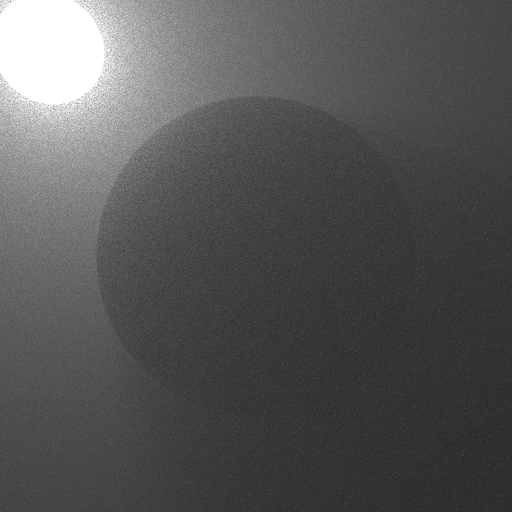
\includegraphics[width=0.48\linewidth]{imgs/volpath_4.png}
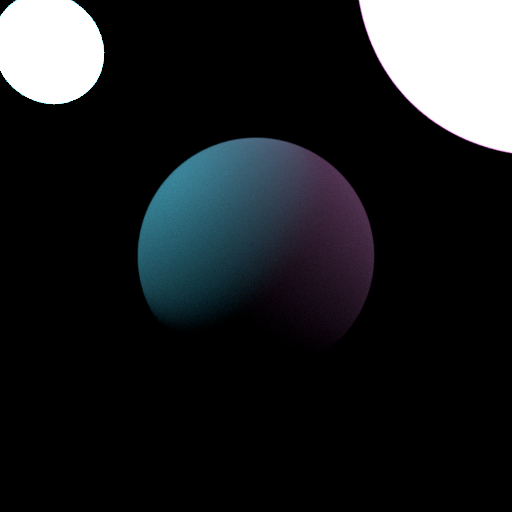
\includegraphics[width=0.48\linewidth]{imgs/volpath_4_2.png}
\caption{Test scenes for our fourth volumetric path tracer. The left scene is similar to the previous test scene in volumetric path tracer 3, but the light source is smaller. The right scene contains a dense volumetric ball floating in the air.}
\label{fig:volpath4}
\end{figure}

\paragraph{Debugging tip.} Implement the method first without multiple importance sampling. Render the previous scene in our third volumetric path tracer. Make sure it converges to the same image.

\paragraph{Question(s) (8\%).} 
\begin{enumerate}
    \item When will next event estimation be more efficient than phase function sampling? In our test scenes, which one is more efficient? Why?
    \item In \lstinline{scenes/volpath_test/volpath_test4_2.xml}, we render a scene with an object composed of dense volume. How does it compare to rendering the object directly with a Lambertian material? Why are they alike or different?
    \item Jim Kajiya famously has predicted in 1991 that \emph{in 10 years, all rendering will be volume rendering}. What do you think that makes him think so? Why hasn't it happened yet?
\end{enumerate}

\paragraph{Task (13\%).} You will implement the algorithm above in the \lstinline{vol_path_tracing_4} function in \lstinline{vol_path_tracing.h}. Test your rendering using the scenes \lstinline{scenes/volpath_test/volpath_test4.xml} and \lstinline{scenes/volpath_test/volpath_test4_2.xml}. You should get images that look like the ones in Figure~\ref{fig:volpath4}.

\section{Multiple monochromatic homogeneous volumes with absorption and multiple-scattering with both phase function sampling and next event estimation, with surface lighting}

We are finally adding surface lighting to our volumetric renderer. This should be much easier compared to the last two parts. So far, whenever we encounter a surface, we use $L_e$ to represent its emission. Adding surface lighting is just replacing $L_e$ with the full rendering equation (that includes transmittance and volumetric scattering). Code-wise, we just need to go through all the places where we sample or evaluate the phase function, and also consider the case where we hit a surface and include the BSDF sampling and evaluation. I will let you figure out the details! 

\begin{figure}
\centering
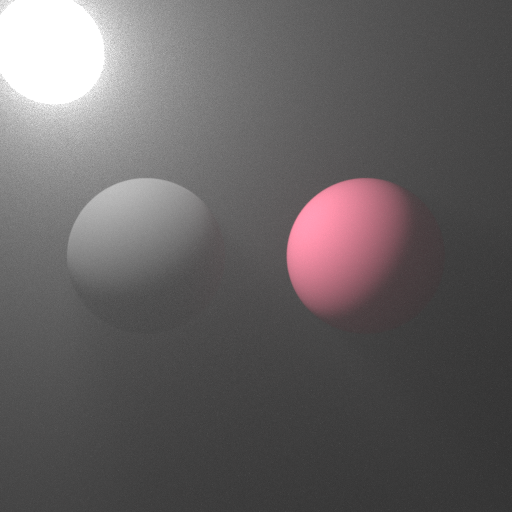
\includegraphics[width=0.48\linewidth]{imgs/volpath_5.png}
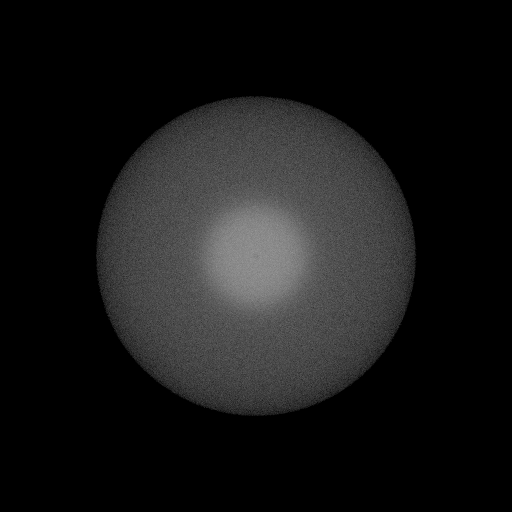
\includegraphics[width=0.48\linewidth]{imgs/volpath_5_2.png}
\caption{Test scenes for our fifth volumetric path tracer. The left scene contains a volumetric ball and an opaque Lambertian ball (with red reflectance). The right scene contains an outer sphere with a dielectric interface and an inner sphere with Lambertian material, and between them is a dense volume.}
\label{fig:volpath5}
\end{figure}

\begin{figure}
\centering
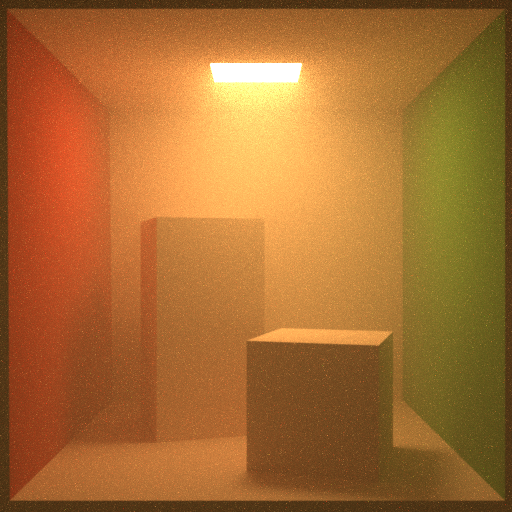
\includegraphics[width=0.48\linewidth]{imgs/volpath_5_cbox.png}
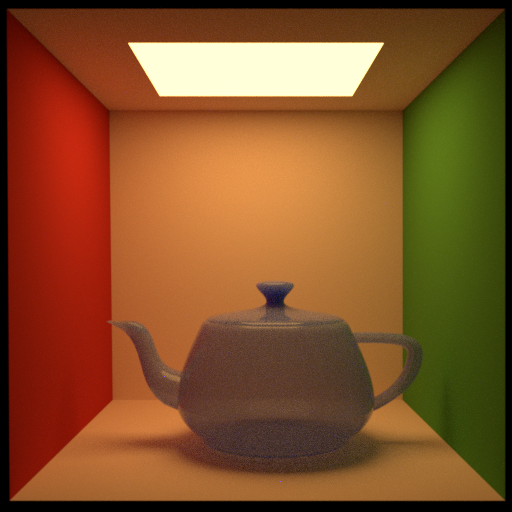
\includegraphics[width=0.48\linewidth]{imgs/volpath_5_cbox_teapot.png}
\caption{Cornell box scenes that we can render with our fifth volumetric path tracer.}
\label{fig:volpath5_cbox}
\end{figure}

\paragraph{Question(s) (8\%).} 
\begin{enumerate}
    \item Play with the index of refraction parameter of the dielectric interface in \\ \lstinline{scenes/volpath_test/volpath_test5_2.xml}. How does that affect appearance? Why?
    \item In the scene \lstinline{scenes/volpath_test/vol_cbox_teapot.xml}, we model the glass teapot as a transparent glass with blue homogeneous medium inside. What is the difference in terms of appearance between this approach and just making the color of the glass blue without any medium inside?
\end{enumerate}

\paragraph{Task (10\%).} You will add surface lighting in the \lstinline{vol_path_tracing_5} function in \lstinline{vol_path_tracing.h}. Test your rendering using the scenes \lstinline{scenes/volpath_test/volpath_test5.xml} and \lstinline{scenes/volpath_test/volpath_test5_2.xml}. You should get images that look like the ones in Figure~\ref{fig:volpath5}. Also check out \lstinline{scenes/volpath_test/vol_cbox.xml} and \lstinline{scenes/volpath_test/vol_cbox_teapot.xml} to see what we can render now (Figure~\ref{fig:volpath5_cbox})!

\section{Multiple chromatic heterogeneous volumes with absorption and multiple-scattering with both phase function sampling and next event estimation, with surface lighting}

We reach the final stage of this homework. This last part is a bit tough due to the mathematicaly complexity (but the implementation isn't that bad), so don't worry too much if you cannot finish it. Even if you don't finish this part, you will still get $90\%$ of the score. But the math is fun and you should try to understand it!

So far, we have been assuming that 1) the volumes are monochromatic, and 2) they are homogeneous. We are going to solve the two problems at once with a super clever idea called \emph{null-scattering}. Let's focus on heterogeneous media first and look at the radiative transfer equation (assuming no volumetric emission):
\begin{equation}
\frac{\mathrm{d}}{\mathrm{d}t}L(\mathbf{p}(t), \omega) = -\sigma_t(\mathbf{p}(t)) L(\mathbf{p}(t), \omega) + \sigma_s(\mathbf{p}(t)) \int_{S^2} \rho(\omega, \omega') L(\mathbf{p}(t), \omega') d\omega',
\end{equation}
with boundary condition $L(\mathbf{p}(t_{\text{hit}}), \omega) = L_{\text{surface}}(\mathbf{p}(t_{\text{hit}}))$ to account for surface lighting.

Integrating over distance, we get our integral volume rendering equation:
\begin{equation}
L(\mathbf{p}(t), \omega) = \int_{0}^{t_{\text{hit}}} T(\mathbf{p}(0), \mathbf{p}(t'))
\left(\sigma_s(\mathbf{p}(t')) \int_{S^2} \rho(\omega, \omega') L(\mathbf{p}(t'), \omega') \mathrm{d}\omega' \right) \mathrm{d}t' + T(\mathbf{p}(0), \mathbf{p}(t_{\text{hit}})) L_{\text{surface}}(\mathbf{p}(t_{\text{hit}})),
\end{equation}
where $T$ is the transmittance:
\begin{equation}
T(\mathbf{p}(0), \mathbf{p}(t')) = \exp\left(-\int_{0}^{t'} \sigma_t\left(\mathbf{p}(t'')\right) \mathrm{d}t'' \right).
\end{equation}

The transmittance has a closed-form when the volume is homogeneous. However when we have heterogeneous volumes (i.e. $\sigma_t$ changes with position), we need to use Monte Carlo to estimate the transmittance. The exponential makes it tricky to do an unbiased estimation: $E[\exp(X)] \neq \exp(E[X])$ for most random variable $X$, where $E$ is expectation. This means that when we have an estimation of the integral $X \approx \int_{0}^{t'} \sigma_t\left(\mathbf{p}(t'') \mathrm{d}t''\right)$, even if $X$ is unbiased ($E[X] = \int_{0}^{t'} \sigma_t\left(\mathbf{p}(t'')\right) \mathrm{d}t''$), the exponentiation of $X$ won't be an unbiased estimation of the exponentiation of the integral.

\paragraph{Homogenized free-flight sampling.} To resolve this, we apply a trick called \emph{homogenization}. That is, we convert the heterogeneous medium into a homogeneous medium by inserting \emph{fake} particles that do not scatter lights. Then we can use the closed-form solution from the homogeneous medium to obtain an answer. Mathematically, we modify the radiative transfer equation as follows:
\begin{equation}
\frac{\mathrm{d}}{\mathrm{d}t}L(\mathbf{p}(t), \omega) = -(\sigma_t(\mathbf{p}(t)) + \sigma_n(\mathbf{p}(t))) L(\mathbf{p}(t), \omega) + \sigma_n(\mathbf{p}(t)) L(\mathbf{p}(t), \omega) + \sigma_s(\mathbf{p}(t)) \int_{S^2} \rho(\omega, \omega') L(\mathbf{p}(t), \omega') d\omega',
\end{equation}
where $\sigma_n$ is the density of the \emph{fake} particles. All we did is to add $-\sigma_n L + \sigma_n L$ to the right-hand side, so we did not alter the values of the radiative transfer equation at all.

Now, if we choose the fake particle density $\sigma_n(\mathbf{p}(t))$ such that $\sigma_t(\mathbf{p}(t)) + \sigma_n(\mathbf{p}(t))$ is a constant for all $t$, then we convert the radiative transfer equation back to a homogeneous medium! 

What constant should we choose? A common choice is the upper bound of $\sigma_t(\mathbf{p}(t))$ for all $t$, so that $\sigma_n(\mathbf{p}(t)) \geq 0$. We call the upper bound the \emph{majorant} ($\sigma_m$). Now we can write the volume integral equation as:
\begin{equation}
\begin{aligned}
L(\mathbf{p}(t), \omega) = &\int_{0}^{t_{\text{hit}}} T_m(\mathbf{p}(0), \mathbf{p}(t'))
\left(\sigma_n(\mathbf{p}(t')) L(\mathbf{p}(t'), \omega) + \sigma_s(\mathbf{p}(t')) \int_{S^2} \rho(\omega, \omega') L(\mathbf{p}(t'), \omega') \mathrm{d}\omega' \right) \mathrm{d}t' + \\
&T_m(\mathbf{p}(0), \mathbf{p}(t_{\text{hit}})) L_{\text{surface}}(\mathbf{p}(t_{\text{hit}})),
\end{aligned}
\end{equation}
where $T_m$ is the \emph{homogenized} transmittance:
\begin{equation}
T_m(\mathbf{p}(0), \mathbf{p}(t')) = \exp\left(-\sigma_m t'\right).
\end{equation}

To evaluate $L$, we importance sample the homogenized transmittance $T_m$. Every time we sample a distance $t'$ based on the homogenized transmittance, three things can happen:
\begin{enumerate}
    \item We hit the surface ($t' \geq t_{\text{hit}}$), and need to compute $L_{\text{surface}}$.
    \item We hit a \emph{real} particle, and need to compute the $S^2$ integral to scatter the particle.
    \item We hit a \emph{fake} particle, and need to keep evaluating $L$ by continuing the ray in a straight line.
\end{enumerate}

The probability that the first event happenning is the same as Equation~\ref{eq:hit_surface_prob}. For the second and third event, we can use whatever probability we like (it's just importance sampling). We will choose the \emph{real} probability to be $\frac{\sigma_t}{\sigma_m}$, and the \emph{fake} probability to be $\frac{\sigma_n}{\sigma_m}$ (a more optimal way to assign the probability is to set the real probability to $\frac{\sigma_s}{\sigma_s + \sigma_n}$, but then it is possible that $\sigma_s + \sigma_n = 0$ and we need to deal with those corner cases, so we opt for simplicity here). We arrive at the classical \emph{delta tracking} (or Woodcock tracking) algorithm~\cite{Woodcock:1965:TGC}.

\paragraph{Homogenized next event estimation.} Next, we need to evaluate the transmittance (instead of importance sampling) for the next event estimation.
We will use the same homogenization trick.
We have the following integral to estimate between two points $\mathbf{p}(0)$ and $\mathbf{p}(t')$:
\begin{equation}
T(\mathbf{p}(0), \mathbf{p}(t')) = T_\mathbf{p}(t') = \exp\left(-\int_{0}^{t'}\sigma_t(\mathbf{p}(t''))\mathrm{d}t''\right).
\end{equation}
We again observe that $T_\mathbf{p}(t')$ is the solution of an ordinary differential equation
\begin{equation}
\begin{aligned}
\frac{\mathrm{d}T_\mathbf{p}\left(t'\right)}{\mathrm{d}t'} &= -\sigma_t(\mathbf{p}(t'))T_\mathbf{p}\left(t'\right) = -\sigma_m T_\mathbf{p}\left(t'\right) + \sigma_n(\mathbf{p}(t))T_\mathbf{p}\left(t'\right). \\
T_\mathbf{p}(0) &= 1
\end{aligned}
\end{equation}
where we homogenize the ODE using the majorant $\sigma_t(\mathbf{p}(t')) = \sigma_m - \sigma_n(\mathbf{p}(t'))$.

To solve this ODE, we apply a change of variable $\tilde{T}_{\mathbf{p}}(t') = \exp\left(\sigma_m t'\right) T_{\mathbf{p}}(t')$. This gives us
\begin{equation}
\begin{aligned}
\frac{\mathrm{d}}{\mathrm{d}t'}\tilde{T}_{\mathbf{p}}(t') &= \frac{\mathrm{d}}{\mathrm{d}t'}\left(\exp\left(\sigma_m t'\right) T_{\mathbf{p}}(t')\right) = \sigma_n(\mathbf{p}(t')) \tilde{T}_{\mathbf{p}}(t') \\
\tilde{T}_{\mathbf{p}}(0) &= 1
\end{aligned}.
\end{equation}

Instead of solving the ODE above using exponentiation (which gives us back the exponential integral), we simply integrate both sides and get $\tilde{T}_{\mathbf{p}}(t') = 1 + \int_0^{t'} \sigma_n(\mathbf{p}(t'')) \tilde{T}_{\mathbf{p}}(t'') \mathrm{d}t''$. Changing the variable back to $T$ from $\tilde{T}$ gives us:
\begin{equation}
\begin{aligned}
T_{\mathbf{p}}(t') = \frac{\tilde{T}_{\mathbf{p}}(t')}{\exp\left(\sigma_m t'\right)} &= \exp\left(-\sigma_m t'\right) \left(1 + \int_{0}^{t'} \exp\left(\sigma_m t''\right) \sigma_n(\mathbf{p}(t'')) T_{\mathbf{p}}(t'') \mathrm{d}t'' \right) \\
&= \exp\left(-\sigma_m t'\right) + \int_{0}^{t'} \exp\left(\sigma_m (t''-t')\right) \sigma_n(\mathbf{p}(t'')) T_{\mathbf{p}}(t'') \mathrm{d}t'',
\end{aligned}
\label{eq:transmittance_recursive_integral}
\end{equation}
and now we have a recursive integral equation that we can directly estimate using Monte Carlo. (we can get an integral that does not involve homogenization nor exponentiation by just integrating both sides of $\frac{\mathrm{d}T_\mathbf{p}\left(t'\right)}{\mathrm{d}t'} = -\sigma_t(\mathbf{p}(t'))T_\mathbf{p}\left(t'\right)$, but Monte Carlo sampling of this integral turns out to be very very slow. See Georgiev et al.'s article for a deeper discussion~\cite{Georgiev:2019:IFV}.) This change of variable trick is called an \emph{exponential integrator} in ODE literature (Google it if you're interested ;).

The Monte Carlo sampler we will apply for solving Equation~\ref{eq:transmittance_recursive_integral} is called the \emph{ratio tracking} method. The idea is to use a path tracing like algorithm with Russian roulette. We notice that the recursive integral is a bit like the rendering equation: we have the \emph{light source term} $\exp\left(-\sigma_m t'\right)$, and the recursive integral $\int_{0}^{t'} \exp\left(\sigma_m (t''-t')\right) \sigma_n(\mathbf{p}(t'')) T_{\mathbf{p}}(t'') \mathrm{d}t''$. 
Starting from $z=t'$, we sample a distance $z_d$ such that $p(z_d) \propto \exp\left(-\sigma_m z_d\right)$ and update $z$. If we reach 0, then we evaluate the light source term. Otherwise, we evaluate the recursive term. One way to think about this is that we hit the fake particle if we choose to evaluate the recursive term. The probability for evaluating the light source term is $\exp\left(-\sigma_m z\right)$ (Equation~\ref{eq:hit_surface_prob}), and the probability density for evaluating the recursive term is $\exp\left(-\sigma_m z_d\right) \sigma_m$. We accumulate these probabilities by multiplying them, while also accounting for the integrand.

\paragraph{Dealing with chromatic media.} Finally, we need to deal with colors. So far, we have been assuming that $\sigma_a$ and $\sigma_s$ are monochromatic, but in practice, they can be RGB colors (or even a vector representing response per wavelength). We deal with this by sampling a channel (R, G, or B) whenever we need to sample distance. Importantly, when computing probability density, we take the average probability density over all channels: this is a form of multiple importance sampling (called the one-sample multiple importance sampling~\cite{Veach:1995:OCS}). To achieve this, we need to keep track of the PDFs of all color channels. Therefore our PDFs have the type \lstinline{Spectrum} instead of \lstinline{Real}.

\paragraph{Multiple importance sampling.} To combine phase function sampling with the next event estimation, we need the PDFs for the ratio tracking (the sequence of decisions we make to evaluate either the recursive term or the source term) during free-flight sampling, and the PDFs of free-flight sampling (the real/fake particle events) during next event estimation. So when evaluating the PDF for one of them, we must also accumulate the PDF of the other. The PDFs of both are products of the homogenized transmittance sampling density $\exp\left(-\sigma_m \Delta_t\right) \sigma_m$ (where $\Delta_t$ is the distance traveled) and the real/fake event probabilities.

Combining all of these, let's look at the pseudo-code. For homogenized free-flight sampling, it looks like this:
\begin{lstlisting}[language=python]
scatter = False
never_scatter = True
transmittance = make_const_spectrum(1)
trans_dir_pdf = make_const_spectrum(1) # PDF for free-flight sampling
trans_nee_pdf = make_const_spectrum(1) # PDF for next event estimation
if in_medium():
  majorant = get_majorant(medium, ray);
  # Sample a channel for sampling
  u = next(rng) # u \in [0, 1]
  channel = clamp(int(u * 3), 0, 2)
  accum_t = 0
  iteration = 0
  while True:
    if majorant[channel] <= 0:
      break
    if iteration >= max_null_collisions:
      break
    t = -log(1 - next(rng)) / majorant[channel]
    dt = t_hit - accum_t
    # Update accumulated distance
    accum_t = min(accum_t + t, t_hit)
    if t < dt: # haven't reached the surface
      # sample from real/fake particle events
      real_prob = sigma_t / majorant
      if next(rng) < real_prob[channel]:
        # hit a "real" particle
        scatter = true
        never_scatter = False
        transmittance *= exp(-majorant * t) / max(majorant)
        trans_dir_pdf *= exp(-majorant * t) * majorant * real_prob / max(majorant)
        # don't need to account for trans_nee_pdf since we scatter
        break
      else:
        # hit a "fake" particle
        transmittance *= exp(-majorant * t) * sigma_n / max(majorant)
        trans_dir_pdf *= exp(-majorant * t) * majorant * (1 - real_prob) / max(majorant)
        trans_nee_pdf *= exp(-majorant * t) * majorant / max(majorant)
    else: # reach the surface
      transmittance *= exp(-majorant * dt)
      trans_dir_pdf *= exp(-majorant * dt)
      trans_nee_pdf *= exp(-majorant * dt)
      break
    iteration += 1
\end{lstlisting}

Two crucial differences between the pseudo code and the math above are:
1) We terminate the loop when the iteration reaches a maximum amount of fake particle collisions 
(default is set to $1000$). While this is not mathematically correct, I found that sometimes
the numerical error can lead to unbounded loops.
2) We divide both transmittance and the PDF with the maximum of the majorant. This is to improve
numerical robustness. Whenever we hit the fake particle, both the transmittance and
the free-flight PDF needs to be multiplied with $\sigma_n$ (note that $\sigma_m (1 - \sigma_t / \sigma_m) = \sigma_n$),
which can be a few hundreds or larger. If we do not normalize these values, the numbers will
quickly blow up and go to infinity.

For the transmittance estimation in next event estimation the pseudo code looks like this:
\begin{lstlisting}[language=python]
p_prime = sample_point_on_light(p)
# Compute transmittance to light. Skip through index-matching shapes.
T_light = make_const_spectrum(1)
p_trans_nee = make_const_spectrum(1)
p_trans_dir = make_const_spectrum(1)
while True:
  shadow_ray = Ray(p, p_prime - p)
  isect = intersect(scene, shadow_ray)
  next_t = distance(p, p_prime)
  if isect:
    next_t = distance(p, isect.position)
    # Account for the transmittance to next_t
    if shadow_medium:
      u = next(rng) # Sample a channel for sampling
      channel = clamp(int(u * 3), 0, 2)
      iteration = 0
      while True:
        if majorant[channel] <= 0:
          break
        if iteration >= max_null_collisions:
          break
        t = -log(1 - next(rng)) / majorant[channel]
        dt = next_t - accum_t
        accum_t = min(accum_t + t, next_t)
        if t < dt:
          # didn't hit the surface, so this is a null-scattering event
          T_light *= exp(-majorant * t) * sigma_n / max(majorant)
          p_trans_nee *= exp(-majorant * t) * majorant / max(majorant)
          real_prob = sigma_t / majorant
          p_trans_dir *= exp(-majorant * t) * majorant * (1 - real_prob) / max(majorant)
          if max(T_light) <= 0: # optimization for places where sigma_n = 0
            break
        else: # hit the surface
          T_light *= exp(-majorant * dt);
          p_trans_nee *= exp(-majorant * dt);
          p_trans_dir *= exp(-majorant * dt);
        iteration += 1
  # same as the previous next event estimation code...
\end{lstlisting}

Notice that whenever we need to compute the Monte Carlo estimate of the transmittance, we need to divide it by the
average PDFs over the RGB channels. For example, when updating the path throughput:
\begin{lstlisting}
current_path_throughput *= (transmittance / avg(trans_dir_pdf))
\end{lstlisting}
Same when computing multiple importance sampling.

\begin{figure}
\centering
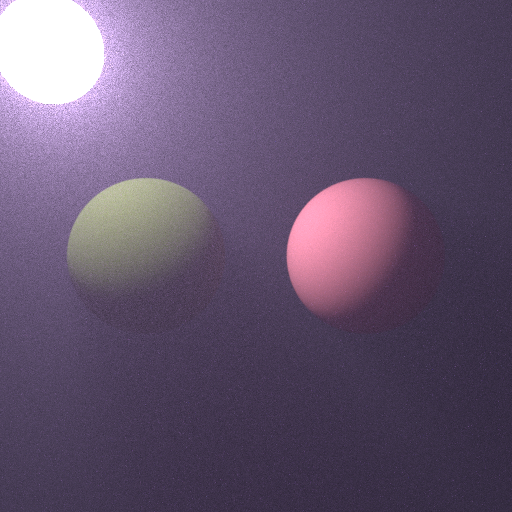
\includegraphics[width=0.48\linewidth]{imgs/volpath_6.png}
\caption{Test scene for our final volumetric path tracer.}
\label{fig:volpath6}
\end{figure}

\begin{figure}
\centering
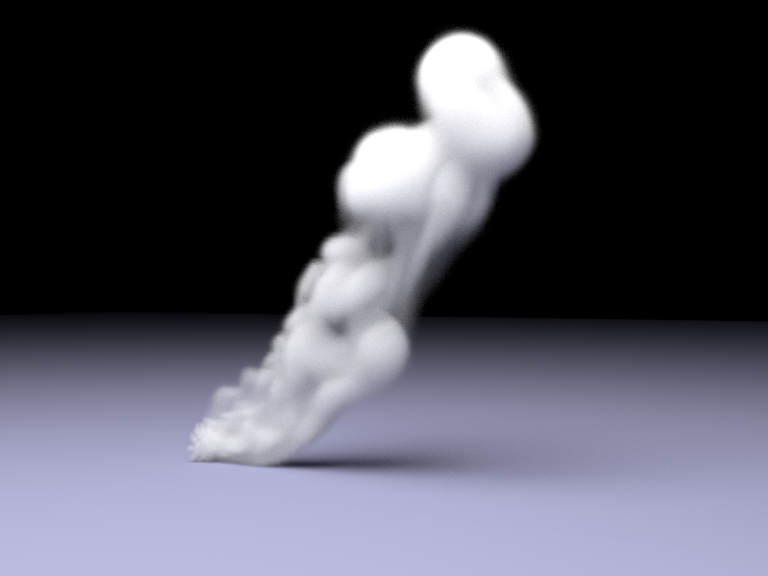
\includegraphics[width=0.48\linewidth]{imgs/hetvol.png}
\caption{Monochromatic heterogeneous volume. Scene data courtesy of Wenzel Jakob.}
\label{fig:hetvol}
\end{figure}

\paragraph{Question (s) (8\%).} 
\begin{enumerate}
    \item For heterogeneous volumes, what kind of distribution of the volume density makes the null scattering efficient/inefficient? Can you think of a way to improve our current sampling scheme in the inefficient case?
    \item How do we make the null-scattering work for emissive volumes? Briefly describe a solution.
    \item Why is it important to have an unbiased solution for volume rendering? Would it be sensible to have something that is biased but faster? How would you do it?
\end{enumerate}

\paragraph{Task (12\%).} You will implement the algorithms above in the \lstinline{vol_path_tracing} function in \lstinline{vol_path_tracing.h}. For getting the majorant, use \lstinline{get_majorant} defined in \lstinline{medium.h}. For accessing \lstinline{max_null_collisions}, use \lstinline{scene.options.max_null_collisions}. Test your rendering using the scenes \lstinline{scenes/volpath_test/volpath_test6.xml} (chromatic homogeneous medium), \lstinline{scenes/volpath_test/hetvol.xml},  \lstinline{scenes/volpath_test/hetvol_colored.xml}. You should get images that look like the ones in Figure~\ref{fig:gallery},~\ref{fig:volpath6}, and~\ref{fig:hetvol}.

\paragraph{Bonus (20\%).} Design some scenes yourself and render them! Consider using Blender to model and export the scene. If you did this bonus, please submit the scene files and rendering and mention it in the README file. For heterogeneous volumes, read \href{https://github.com/BachiLi/lajolla_public/blob/main/src/volume.cpp}{volume.cpp} for the file format. You may find the \href{https://github.com/mitsuba-renderer/mitsuba2-vdb-converter}{Mitsuba 2 VDB converter} to be useful, though I haven't used it myself.

\bibliographystyle{plain}
\bibliography{refs}

\end{document}